\documentclass{tufte-handout}\usepackage[]{graphicx}\usepackage[]{xcolor}
% maxwidth is the original width if it is less than linewidth
% otherwise use linewidth (to make sure the graphics do not exceed the margin)
\makeatletter
\def\maxwidth{ %
  \ifdim\Gin@nat@width>\linewidth
    \linewidth
  \else
    \Gin@nat@width
  \fi
}
\makeatother

\definecolor{fgcolor}{rgb}{0.345, 0.345, 0.345}
\newcommand{\hlnum}[1]{\textcolor[rgb]{0.686,0.059,0.569}{#1}}%
\newcommand{\hlstr}[1]{\textcolor[rgb]{0.192,0.494,0.8}{#1}}%
\newcommand{\hlcom}[1]{\textcolor[rgb]{0.678,0.584,0.686}{\textit{#1}}}%
\newcommand{\hlopt}[1]{\textcolor[rgb]{0,0,0}{#1}}%
\newcommand{\hlstd}[1]{\textcolor[rgb]{0.345,0.345,0.345}{#1}}%
\newcommand{\hlkwa}[1]{\textcolor[rgb]{0.161,0.373,0.58}{\textbf{#1}}}%
\newcommand{\hlkwb}[1]{\textcolor[rgb]{0.69,0.353,0.396}{#1}}%
\newcommand{\hlkwc}[1]{\textcolor[rgb]{0.333,0.667,0.333}{#1}}%
\newcommand{\hlkwd}[1]{\textcolor[rgb]{0.737,0.353,0.396}{\textbf{#1}}}%
\let\hlipl\hlkwb

\usepackage{framed}
\makeatletter
\newenvironment{kframe}{%
 \def\at@end@of@kframe{}%
 \ifinner\ifhmode%
  \def\at@end@of@kframe{\end{minipage}}%
  \begin{minipage}{\columnwidth}%
 \fi\fi%
 \def\FrameCommand##1{\hskip\@totalleftmargin \hskip-\fboxsep
 \colorbox{shadecolor}{##1}\hskip-\fboxsep
     % There is no \\@totalrightmargin, so:
     \hskip-\linewidth \hskip-\@totalleftmargin \hskip\columnwidth}%
 \MakeFramed {\advance\hsize-\width
   \@totalleftmargin\z@ \linewidth\hsize
   \@setminipage}}%
 {\par\unskip\endMakeFramed%
 \at@end@of@kframe}
\makeatother

\definecolor{shadecolor}{rgb}{.97, .97, .97}
\definecolor{messagecolor}{rgb}{0, 0, 0}
\definecolor{warningcolor}{rgb}{1, 0, 1}
\definecolor{errorcolor}{rgb}{1, 0, 0}
\newenvironment{knitrout}{}{} % an empty environment to be redefined in TeX

\usepackage{alltt}

%\geometry{showframe}% for debugging purposes -- displays the margins
\usepackage{graphics}
\usepackage{graphicx}
\usepackage{xcolor}
\usepackage{hyperref}
\hypersetup{colorlinks=true, linkcolor=blue, citecolor=blue, linktocpage}
\usepackage{multicol}
\usepackage{comment}
\usepackage{natbib}
\usepackage{amsmath}
\usepackage{float}
\usepackage{longtable}
\usepackage{booktabs}

\newenvironment{itemize*}%
  {\begin{itemize}%
    \setlength{\itemsep}{0pt}%
    \setlength{\parskip}{0pt}}%
  {\end{itemize}}
	
\newenvironment{enumerate*}%
  {\begin{enumerate}%
    \setlength{\itemsep}{0pt}%
    \setlength{\parskip}{0pt}}%
  {\end{enumerate}}
	
	\newenvironment{description*}%
  {\begin{description}%
    \setlength{\itemsep}{0pt}%
    \setlength{\parskip}{0pt}}%
  {\end{description}}


\title{Flood Interval Analysis}
\author{EA030}
\date{\today~ver. 0.12}
\setkeys{Gin}{width=\linewidth,totalheight=\textheight,keepaspectratio}
% \graphicspath{{graphics/}}



% \SweaveOpts{prefix.string=graphics/plot} % Created a "graphics" subdirectory to 

\setsidenotefont{\color{blue}}
% \setcaptionfont{hfont commandsi}
% \setmarginnotefont{\color{blue}}
% \setcitationfont{\color{gray}}
\IfFileExists{upquote.sty}{\usepackage{upquote}}{}
\begin{document}

\maketitle% this prints the handout title, author, and date
\begin{abstract}
\noindent 
This handout provides an overview of hydrology, focusing on the USGS streamgaging network and the analysis of flood intervals. It covers the basics of hydrology, the significance of stream flow hydrographs, and the concept of flood return intervals. The handout also includes practical examples and visualizations to illustrate these concepts.
\end{abstract}

% Setting up the margins, etc for R


\section{Hydrology Basics}

Hydrology is the scientific study of the movement, distribution, and quality of water on Earth. Its roots trace back to ancient civilizations such as Mesopotamia, Egypt, India, and China, where early societies managed water for agriculture, transportation, and flood control using observational knowledge and basic engineering like canals and embankments.

Hydrology began to formalize as a science in the 17th and 18th centuries with pioneers like Pierre Perrault and Edmund Halley, who quantified rainfall and streamflow. By the 19th century, the rise of civil engineering demanded more precise understanding of water systems for designing infrastructure. Today, hydrology is an interdisciplinary field integrating tools like GIS, remote sensing, and computer models to address modern challenges such as flood risk, water security, and climate change.

\subsection{USGS Stations and Methods}

The United States Geological Survey (USGS) plays a central role in monitoring water resources across the country. As part of its mission to provide impartial scientific information about the natural environment, the USGS operates one of the world’s most extensive and long-standing networks of streamgages, which are used to monitor river and streamflow conditions in real time.

The USGS streamgaging network consists of over 10,000 active stations located throughout the United States, including Alaska, Hawaii, and U.S. territories. These stations collect continuous data on stream discharge, stage (water height), temperature, and sometimes sediment or water quality. Many stations transmit data via satellite or radio every 15 to 60 minutes, making real-time information publicly available through the USGS National Water Information System (NWIS).

This network supports a wide range of applications, including flood forecasting, drought monitoring, water resource management, ecological studies, infrastructure design, and emergency response. Federal, state, and local agencies, as well as private sector users and researchers, rely heavily on USGS data for planning and decision-making.

\begin{marginfigure}
	\centering
		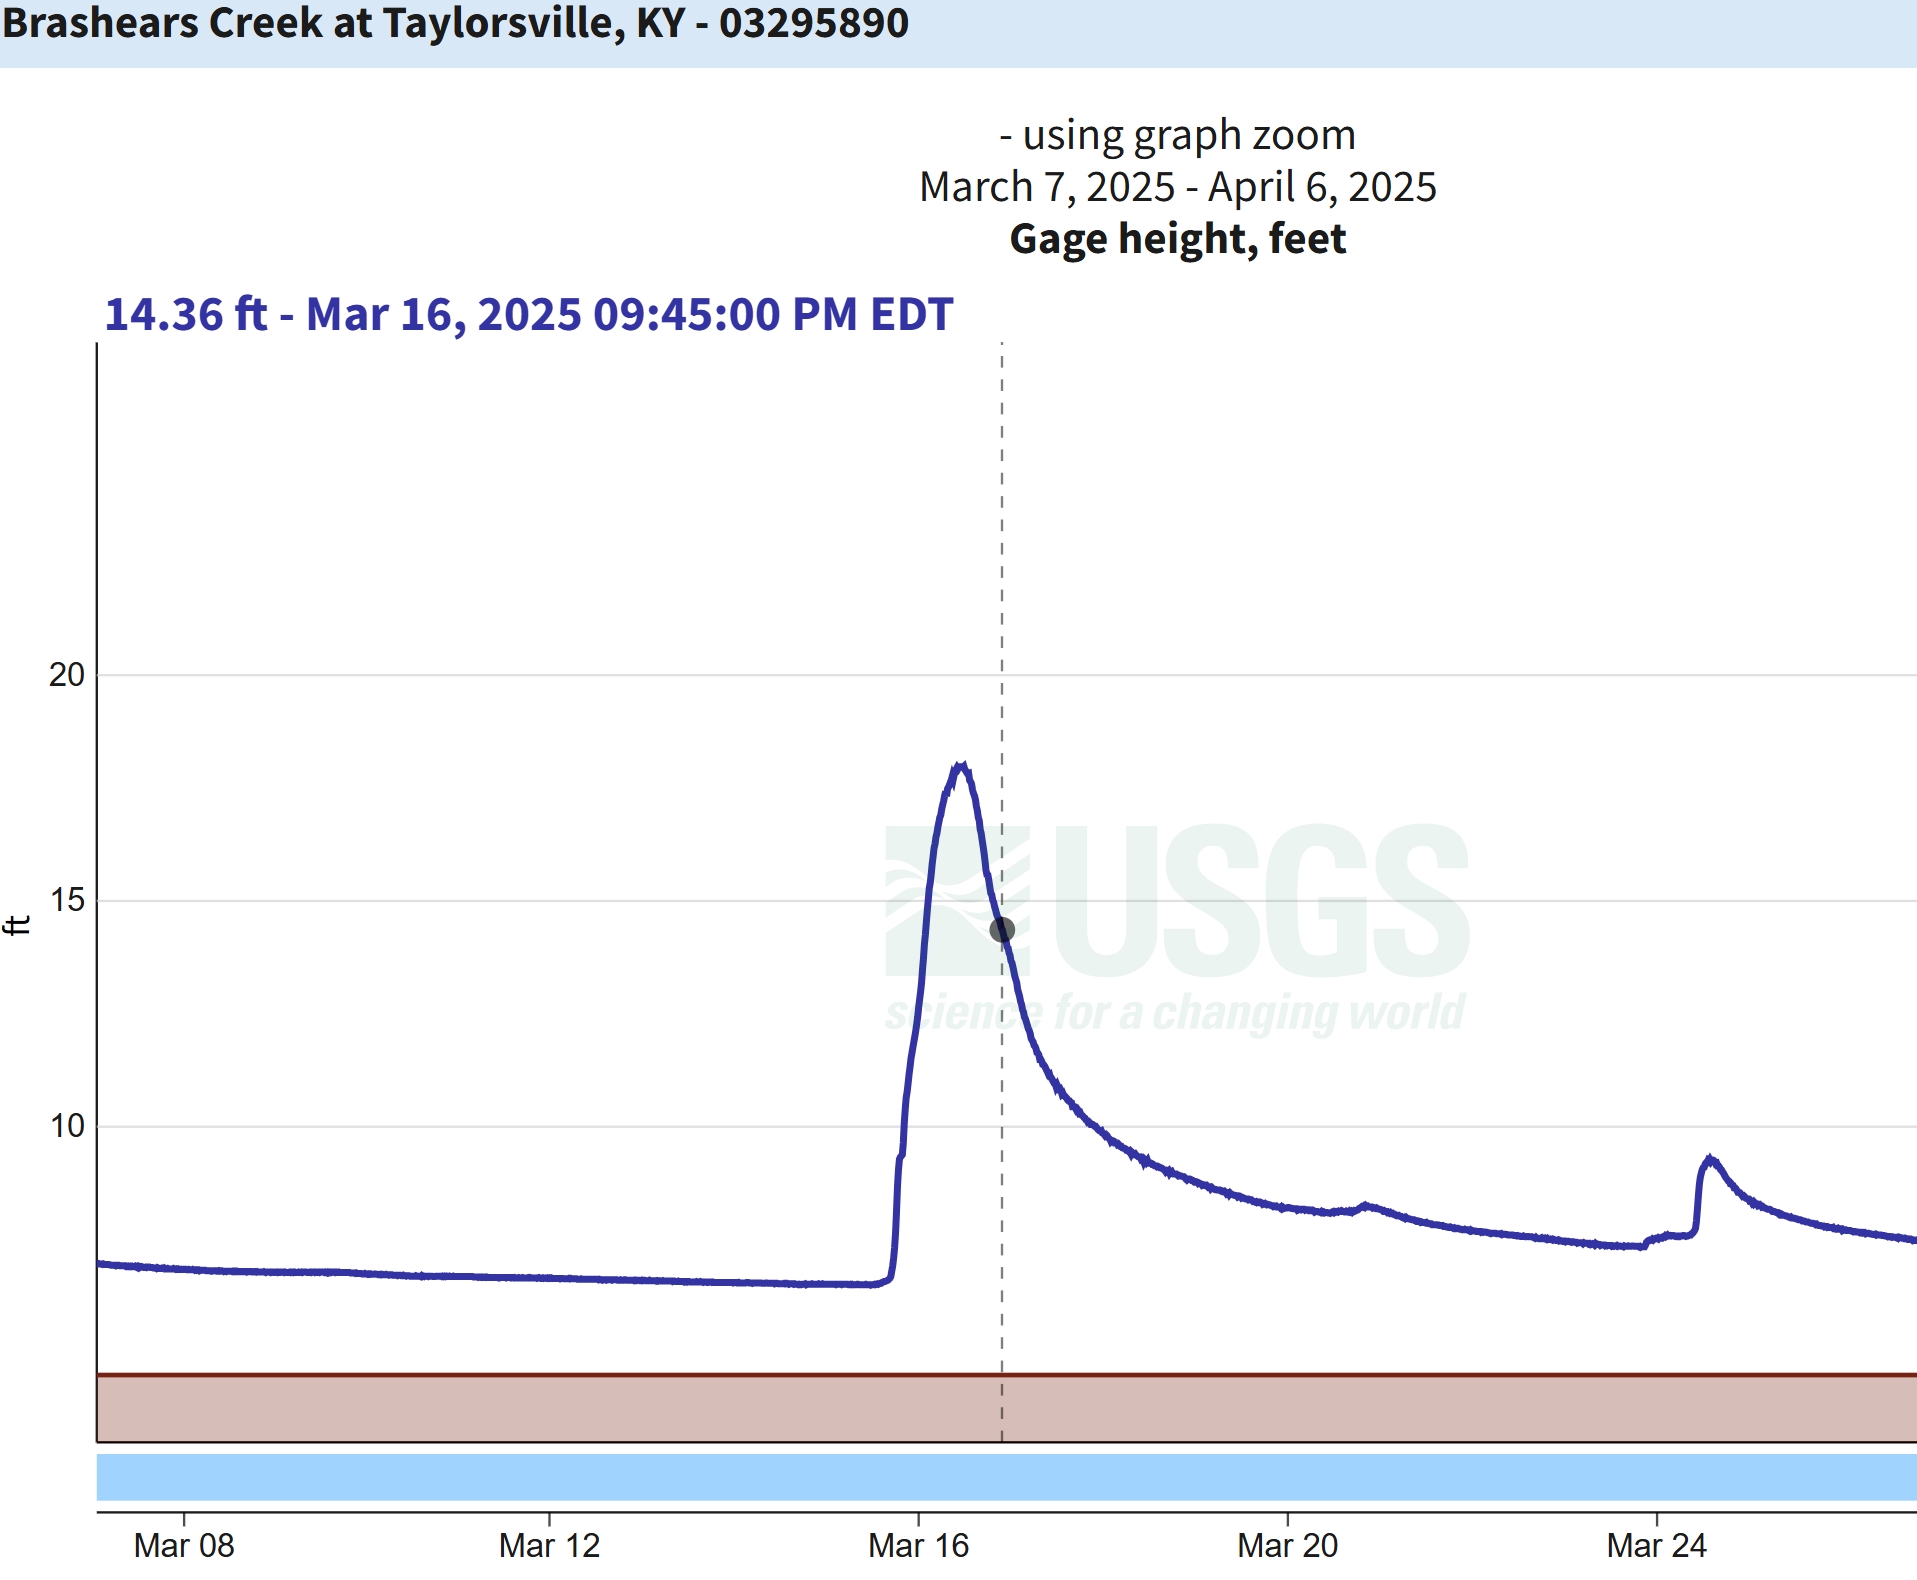
\includegraphics[width=1.00\textwidth]{figure/Gauge_height.png}
		\caption{Gauge Height}
	\label{fig:gauge_ht}
\end{marginfigure}

\subsection{Stream Flow (Discharge) Hydrograph}

A hydrograph displays how river discharge responds to a rainfall event. Its key components include:

\begin{itemize}
  \item \textbf{Rising Limb:} The initial increase in discharge as rainfall runoff enters the river system.
  \item \textbf{Peak Discharge:} The maximum flow rate reached during the event, often corresponding to flood risk.
  \item \textbf{Lag Time:} The delay between peak rainfall and peak discharge, influenced by land use and basin characteristics.
  \item \textbf{Falling Limb:} The decline in flow as water drains away and returns to normal levels.
  \item \textbf{Base Flow:} The underlying groundwater-fed flow present before and after the storm.
\end{itemize}

\begin{marginfigure}
	\centering
		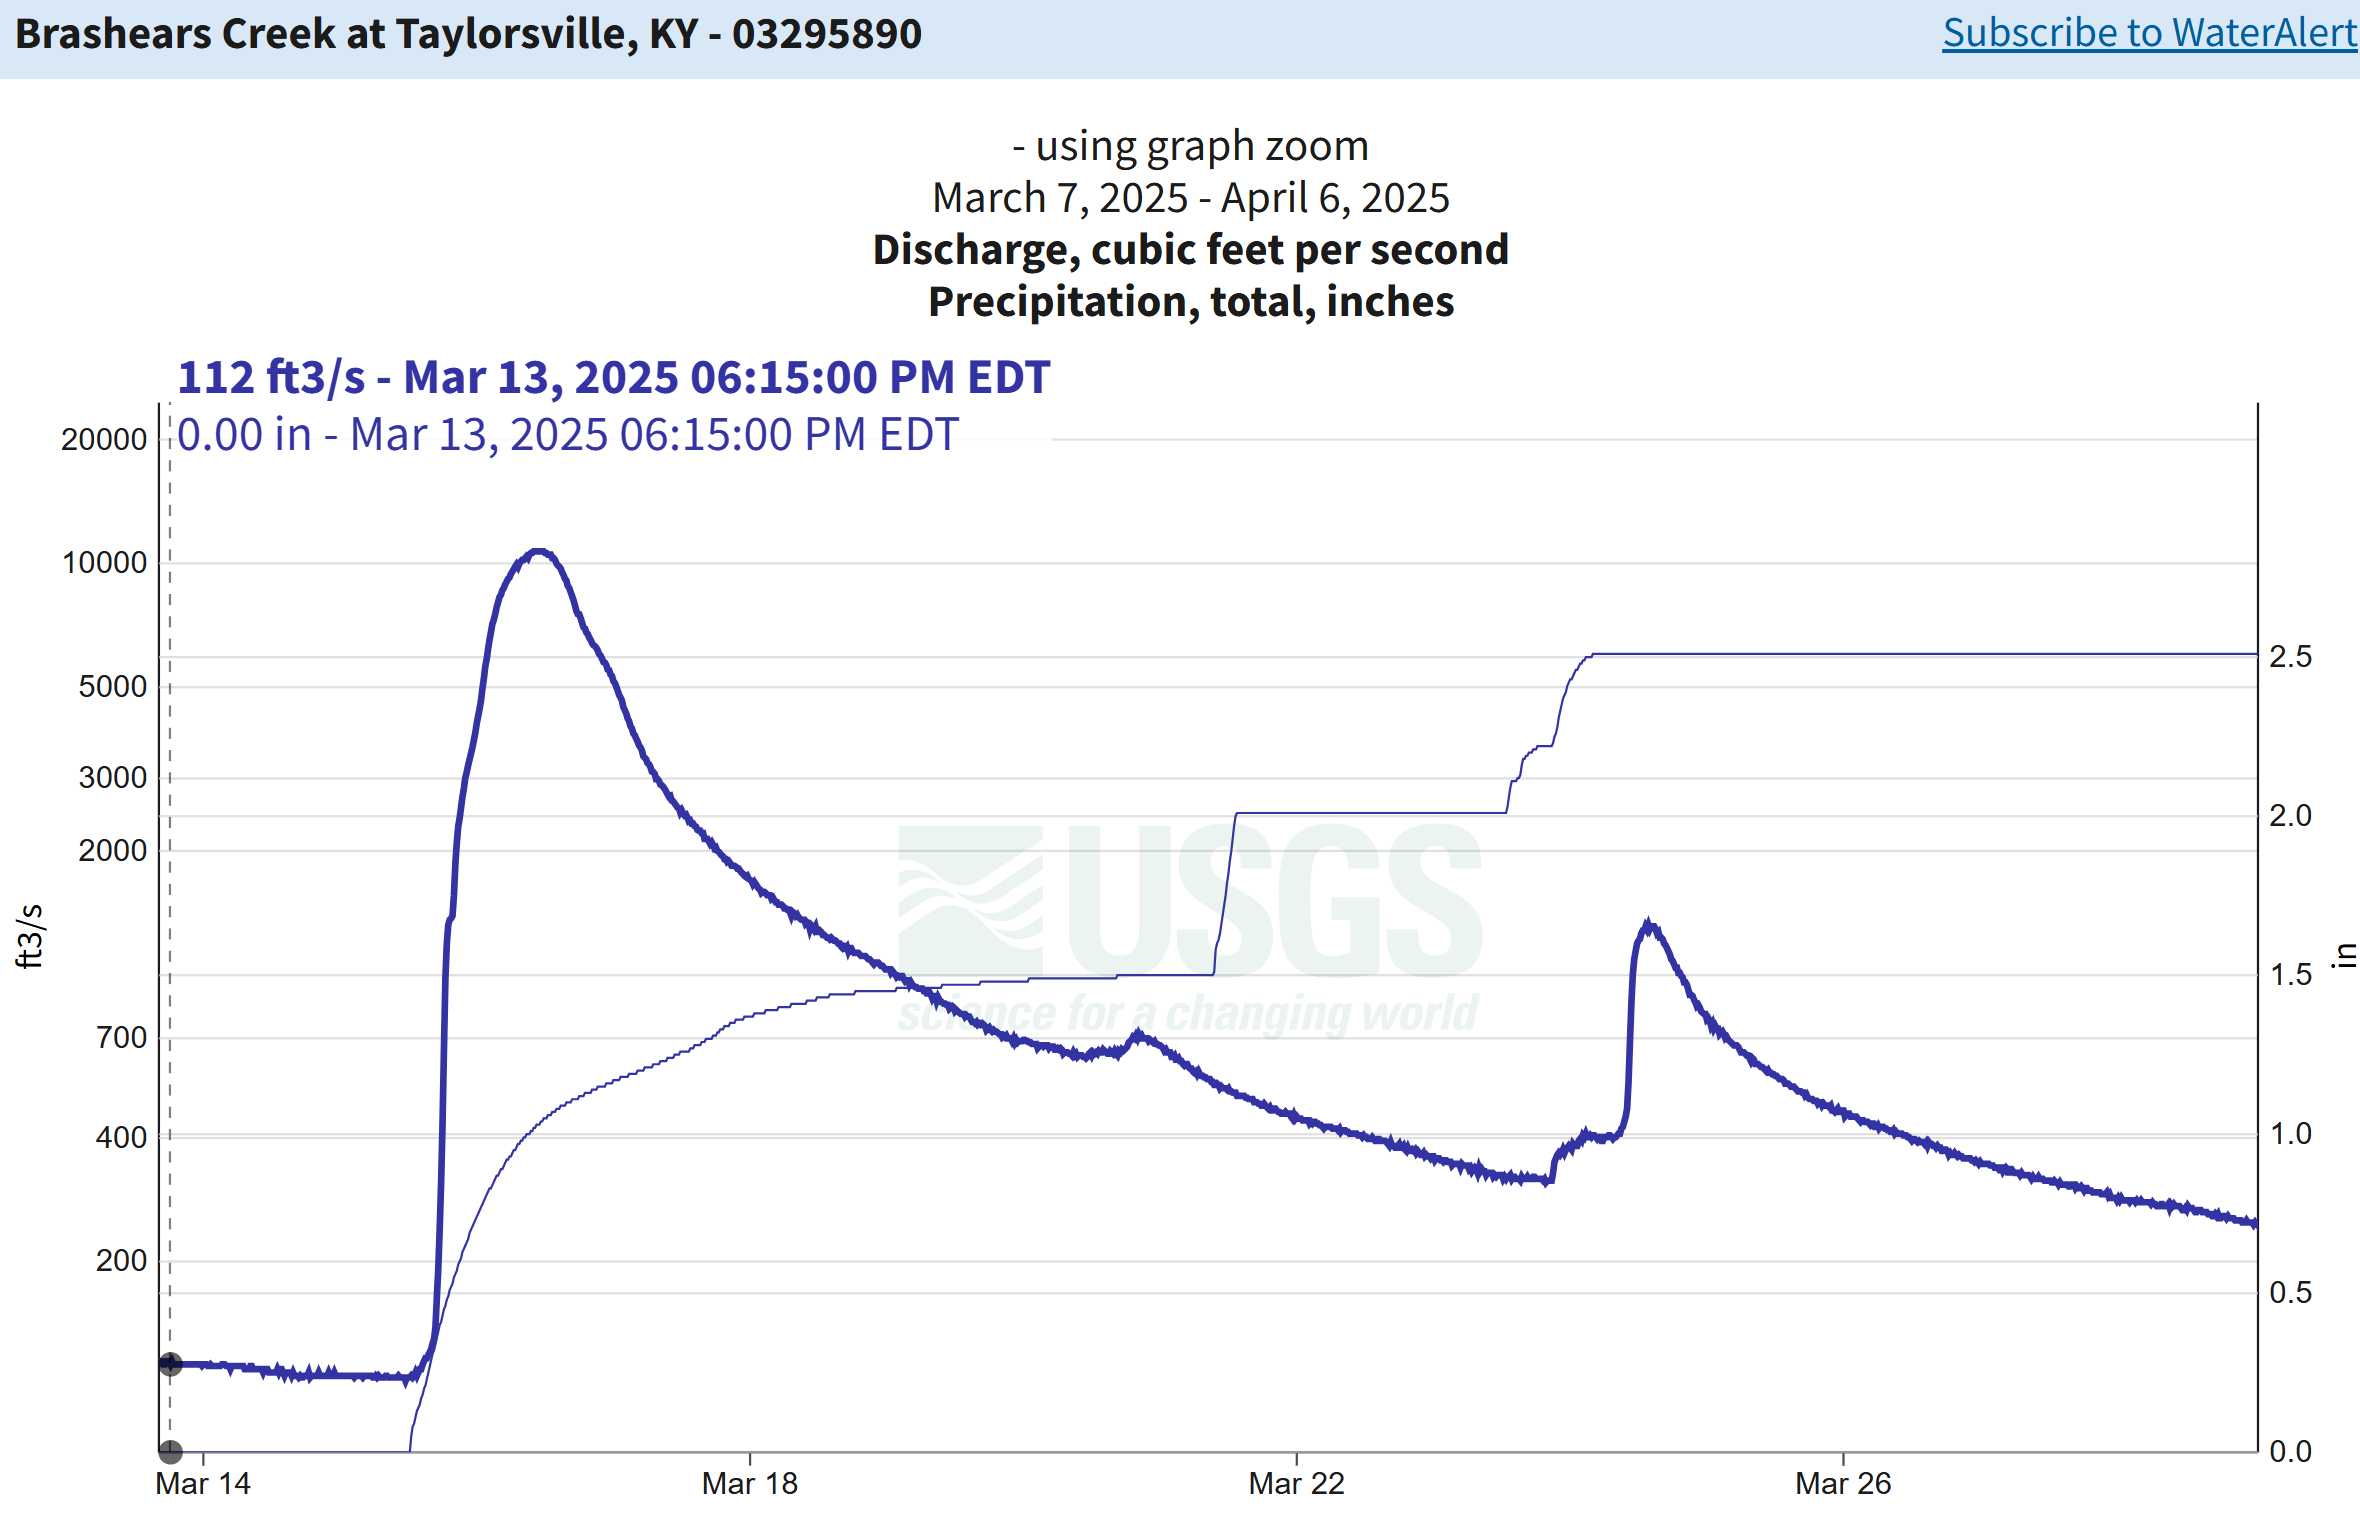
\includegraphics[width=1.00\textwidth]{figure/Discharge.png}
		\caption{Discharge (cubic feet per second) at USGS streamgage 03295890, Brashears Creek at Taylorsville, KY. The hydrograph shows the response of streamflow to a rainfall event on April 5, 2025. The rising limb indicates increasing discharge as runoff enters the river system, while the peak discharge represents the maximum flow rate reached during the event. The falling limb shows the decline in flow as water drains away and returns to normal levels. Base flow is the underlying groundwater-fed flow present before and after the storm. The gauge height is also shown in Figure \ref{fig:gauge_ht}.}
	\label{fig:discharge}
\end{marginfigure}


\subsection{Flood Return Interval}

lood intervals, also known as return periods, estimate how often extreme flood events are likely to occur. These estimates are critical for evaluating flood risk and informing infrastructure design, emergency planning, and land-use decisions. By understanding flood frequency, communities can build safer systems and reduce vulnerability to damaging events.

Return periods are used in engineering and environmental planning. Civil engineers design infrastructure like bridges and dams based on specific flood intervals (e.g., 100-year floods). Urban planners and insurance programs such as FEMA's National Flood Insurance Program use them to guide development and define hazard zones. Scientists also apply flood interval data to study ecosystems and assess climate-related changes in flood behavior.

\begin{figure}
	\centering
		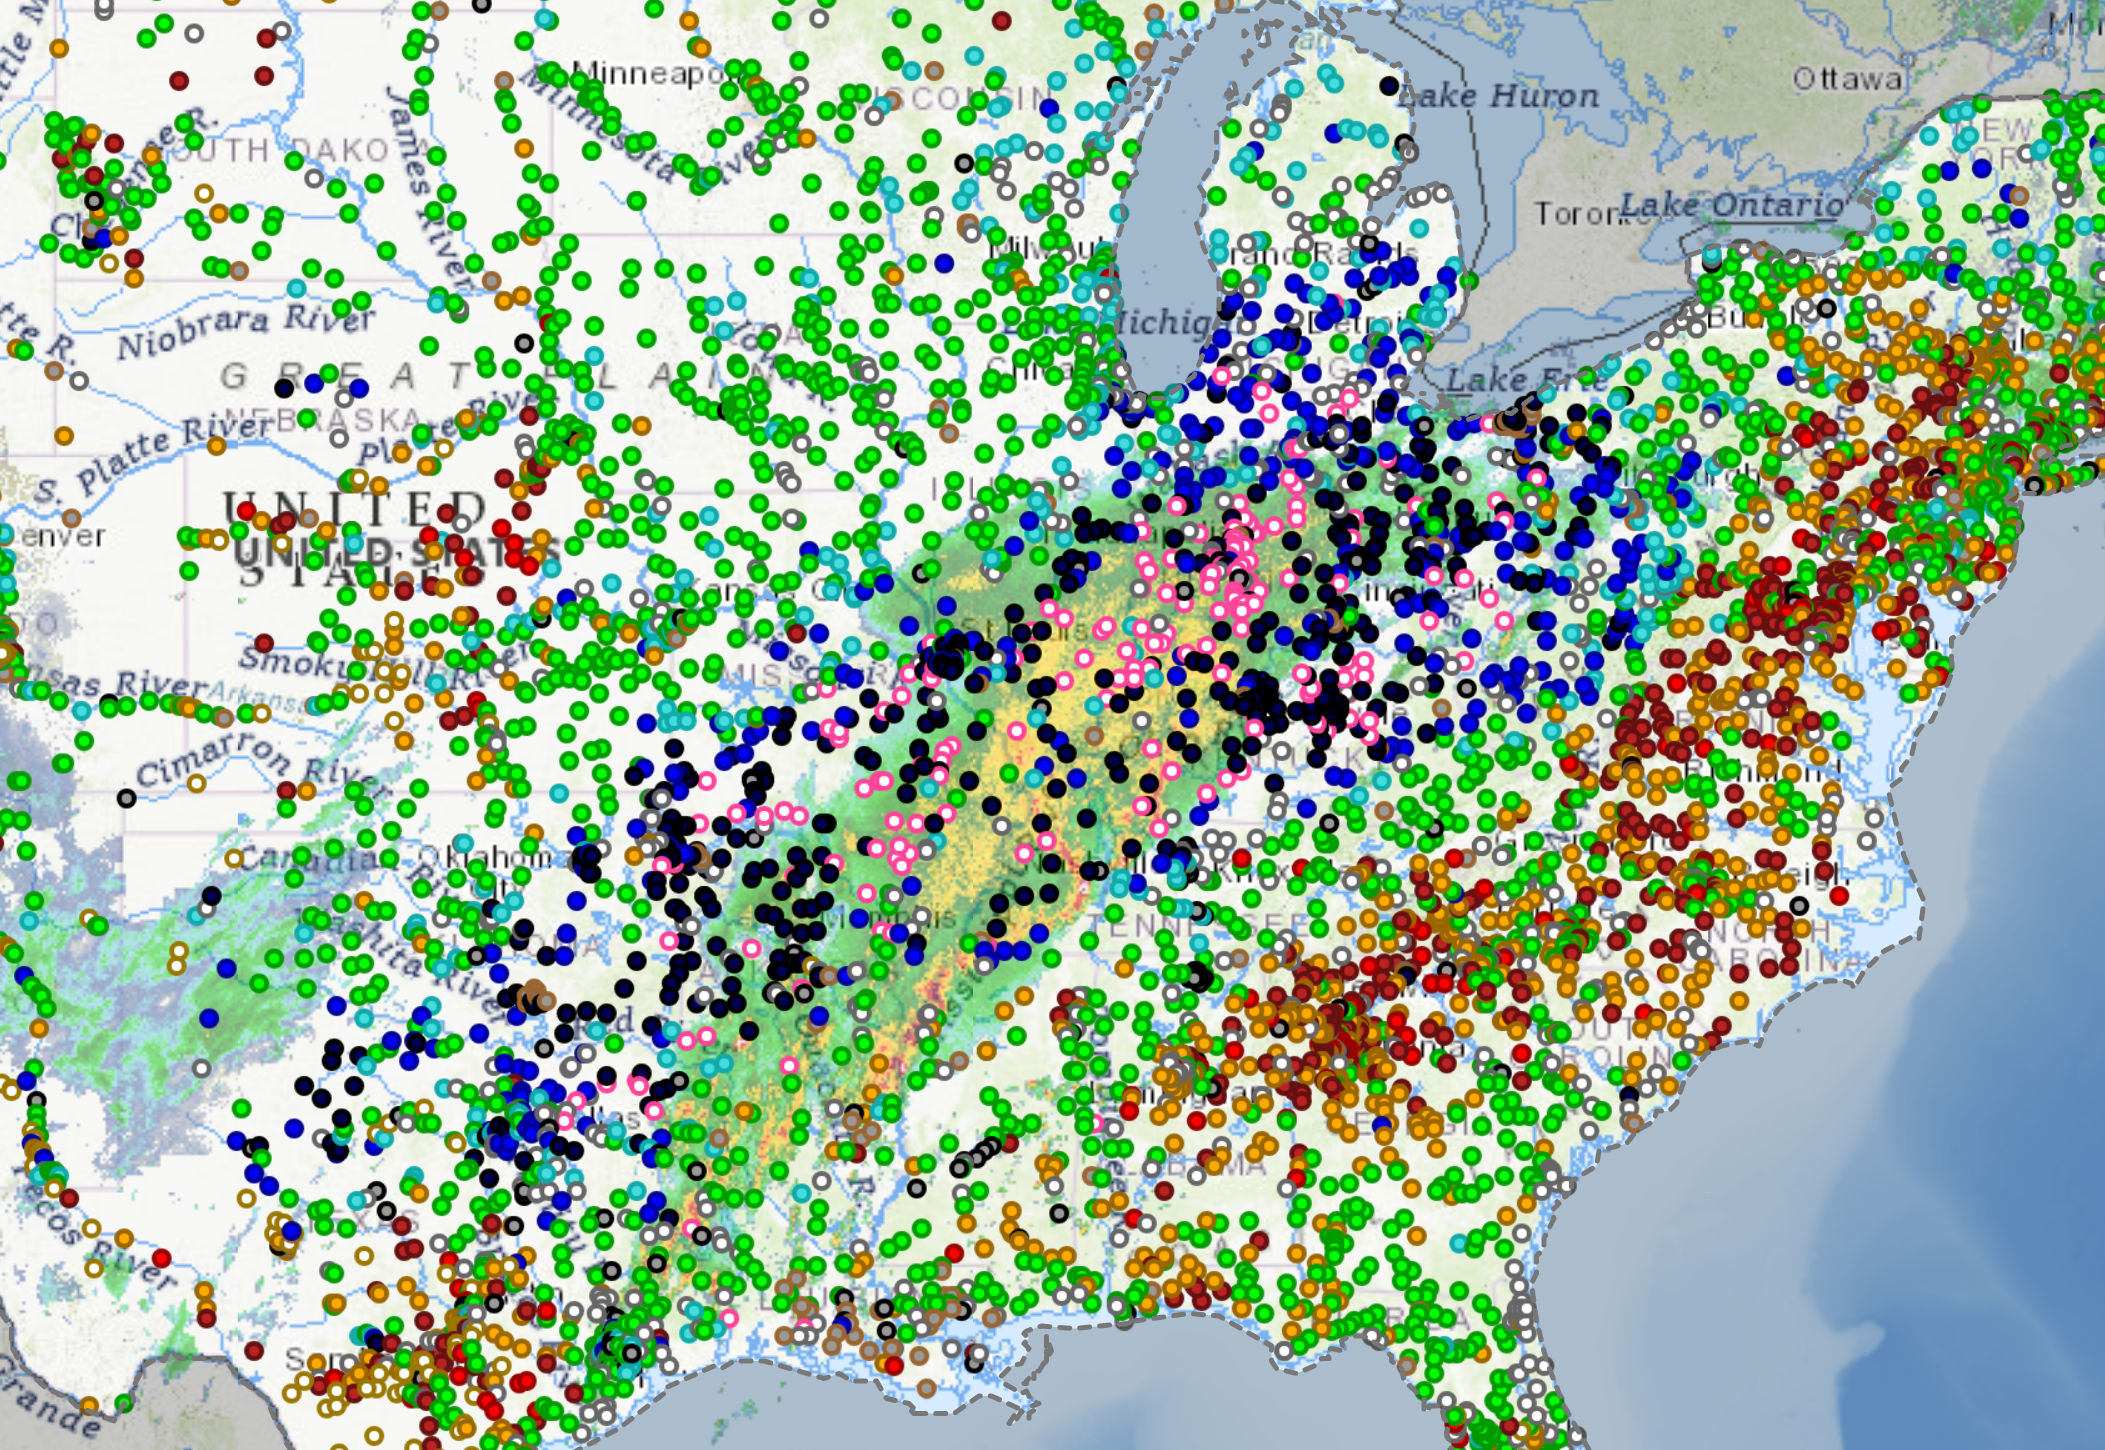
\includegraphics[width=1.00\textwidth]{figure/USGS_Discharge_20250405.png}
		\caption{USGS National Water Dashboard -- Realtime Streamflow, April 5, 2025. Back dots signinify highest discharge on record as of access date. Open pink circles signify flood risks.}
	\label{fig:USGS_Discharge_20250405}
\end{figure}


\section{Methods for Estimating Flood Intervals}

There are several methods used in hydrology to estimate flood intervals or return periods. These methods vary in complexity and applicability depending on the available data and purpose. Below are some of the most common approaches:

\subsection{1. Empirical Method (Plotting Position Formula)}

This is the simplest method and involves ranking annual peak discharges and applying a plotting position, where the return period \( T \) is defined as:

\[
T = \frac{n + 1}{m}
\]


\noindent Where:
\begin{itemize*}
  \item \( n \) is the number of years of data
  \item \( m \) is the rank (1 = largest)
\end{itemize*}

This method does not assume any underlying distribution.

\subsection{2. Gumbel Distribution (Extreme Value Type I)}

A commonly used theoretical distribution for modeling annual maxima is the Gumbel distribution. The return period is related to the probability of exceedance \( P \) as:

\[
P = \frac{1}{T}
\]

The Gumbel cumulative distribution function (CDF) is:

\[
F(x) = \exp\left[-\exp\left(-\frac{x - \mu}{\beta}\right)\right]
\]

Where \( \mu \) is the location parameter and \( \beta \) is the scale parameter. These can be estimated using method of moments or maximum likelihood.

\subsection{3. Log-Pearson Type III Distribution}

This method is widely recommended in the United States for flood frequency analysis. It applies a Pearson Type III distribution to the log-transformed discharge data. The procedure involves:

\begin{itemize*}
  \item Taking the logarithm of the discharge data
  \item Calculating the mean, standard deviation, and skewness
  \item Using these to estimate quantiles for different return periods
\end{itemize*}

\begin{knitrout}
\definecolor{shadecolor}{rgb}{0.969, 0.969, 0.969}\color{fgcolor}\begin{kframe}
\begin{alltt}
\hlcom{# Load necessary library}
\hlkwa{if} \hlstd{(}\hlopt{!}\hlkwd{require}\hlstd{(e1071))} \hlkwd{install.packages}\hlstd{(}\hlstr{"e1071"}\hlstd{,} \hlkwc{dependencies} \hlstd{=} \hlnum{TRUE}\hlstd{)}
\end{alltt}


{\ttfamily\noindent\itshape\color{messagecolor}{\#\# Loading required package: e1071}}\begin{alltt}
\hlkwd{library}\hlstd{(e1071)}  \hlcom{# for skewness function}

\hlcom{# Step 1: Input annual peak discharge data (in m^3/s)}
\hlstd{discharge} \hlkwb{<-} \hlkwd{c}\hlstd{(}\hlnum{400}\hlstd{,} \hlnum{520}\hlstd{,} \hlnum{610}\hlstd{,} \hlnum{700}\hlstd{,} \hlnum{650}\hlstd{,} \hlnum{720}\hlstd{,} \hlnum{800}\hlstd{,} \hlnum{750}\hlstd{,} \hlnum{680}\hlstd{,} \hlnum{670}\hlstd{)}

\hlcom{# Step 2: Log-transform the discharge data}
\hlstd{logQ} \hlkwb{<-} \hlkwd{log10}\hlstd{(discharge)}

\hlcom{# Step 3: Compute statistics of log-values}
\hlstd{mean_logQ} \hlkwb{<-} \hlkwd{mean}\hlstd{(logQ)}
\hlstd{sd_logQ}   \hlkwb{<-} \hlkwd{sd}\hlstd{(logQ)}
\hlstd{skew_logQ} \hlkwb{<-} \hlkwd{skewness}\hlstd{(logQ)}

\hlcom{# Step 4: Define return periods and calculate exceedance probabilities}
\hlstd{T} \hlkwb{<-} \hlkwd{c}\hlstd{(}\hlnum{2}\hlstd{,} \hlnum{5}\hlstd{,} \hlnum{10}\hlstd{,} \hlnum{25}\hlstd{,} \hlnum{50}\hlstd{,} \hlnum{100}\hlstd{)}              \hlcom{# Return periods}
\hlstd{P} \hlkwb{<-} \hlnum{1} \hlopt{-} \hlnum{1} \hlopt{/} \hlstd{T}                             \hlcom{# Exceedance probability}
\hlstd{z} \hlkwb{<-} \hlkwd{qnorm}\hlstd{(P)}                              \hlcom{# Standard normal variate}

\hlcom{# Step 5: Apply Log-Pearson Type III quantile formula}
\hlstd{K} \hlkwb{<-} \hlstd{z} \hlopt{+} \hlstd{( (z}\hlopt{^}\hlnum{2} \hlopt{-} \hlnum{1}\hlstd{)} \hlopt{*} \hlstd{skew_logQ )} \hlopt{/} \hlnum{6}    \hlcom{# Pearson III frequency factor}

\hlstd{logQ_est} \hlkwb{<-} \hlstd{mean_logQ} \hlopt{+} \hlstd{K} \hlopt{*} \hlstd{sd_logQ}       \hlcom{# Estimated logQ}
\hlstd{Q_est} \hlkwb{<-} \hlnum{10}\hlopt{^}\hlstd{logQ_est}                      \hlcom{# Convert back to original scale}

\hlcom{# Combine results in a table}
\hlstd{lp3_results} \hlkwb{<-} \hlkwd{data.frame}\hlstd{(}
  \hlkwc{Return_Period} \hlstd{= T,}
  \hlkwc{Exceedance_Prob} \hlstd{=} \hlkwd{round}\hlstd{(P,} \hlnum{4}\hlstd{),}
  \hlkwc{Discharge_Estimate} \hlstd{=} \hlkwd{round}\hlstd{(Q_est,} \hlnum{2}\hlstd{)}
\hlstd{)}
\end{alltt}
\end{kframe}
\end{knitrout}

\begin{knitrout}
\definecolor{shadecolor}{rgb}{0.969, 0.969, 0.969}\color{fgcolor}\begin{kframe}
\begin{verbatim}
## % latex table generated in R 4.2.2 by xtable 1.8-4 package
## % Sat Apr  5 21:36:29 2025
## \begin{table}[ht]
## \centering
## \begin{tabular}{rrrr}
##   \hline
##  & Return\_Period & Exceedance\_Prob & Discharge\_Estimate \\ 
##   \hline
## 1 & 2.00 & 0.50 & 663.81 \\ 
##   2 & 5.00 & 0.80 & 766.28 \\ 
##   3 & 10.00 & 0.90 & 808.48 \\ 
##   4 & 25.00 & 0.96 & 842.30 \\ 
##   5 & 50.00 & 0.98 & 857.23 \\ 
##   6 & 100.00 & 0.99 & 865.72 \\ 
##    \hline
## \end{tabular}
## \end{table}
\end{verbatim}
\end{kframe}
\end{knitrout}

\subsection{4. Bayesian Methods}

Bayesian approaches allow incorporating prior information and uncertainty in parameter estimates. They are especially useful for short or regional datasets and are implemented via MCMC simulations.

\subsection{5. Regional Frequency Analysis (RFA)}

Instead of analyzing one site in isolation, RFA uses data from multiple similar sites in a region to improve flood frequency estimates. The Index Flood method is a popular RFA technique.

\subsection{6. Generalized Extreme Value (GEV) Distribution}

GEV unifies the Gumbel, Fr\'{e}échet, and Weibull families under one formulation:

\[
F(x) = \exp\left\{ -\left[ 1 + \xi \left(\frac{x - \mu}{\sigma} \right) \right]^{-1/\xi} \right\}
\]

Where:
\begin{itemize*}
  \item \( \mu \) is the location
  \item \( \sigma \) is the scale
  \item \( \xi \) is the shape parameter
\end{itemize*}


These methods are often evaluated based on goodness-of-fit tests, diagnostic plots, and expert judgment.

\section{Using R to Estimate Flood Return Invervals}

\subsection{Annual Peak Flow}

\begin{knitrout}
\definecolor{shadecolor}{rgb}{0.969, 0.969, 0.969}\color{fgcolor}\begin{kframe}
\begin{alltt}
\hlcom{# Eel River Max Dishcharge for USGS Record}
\hlkwd{library}\hlstd{(fields)}
\hlcom{# Use Stream_Hydrography_Analysis to create Eel.df}

\hlcom{# Find Yearly Max flow...}

\hlstd{Eel}\hlopt{$}\hlstd{year} \hlkwb{<-} \hlkwd{as.Date}\hlstd{(Eel}\hlopt{$}\hlstd{date,} \hlstr{"%Y"}\hlstd{)}
\hlstd{Eel}\hlopt{$}\hlstd{maxq} \hlkwb{<-} \hlnum{NA}


\hlkwd{aggregate}\hlstd{(Eel}\hlopt{$}\hlstd{Discharge,} \hlkwd{list}\hlstd{(Eel}\hlopt{$}\hlstd{year), max)} \hlkwb{->} \hlstd{tmp}
\hlkwd{names}\hlstd{(tmp)} \hlkwb{<-} \hlkwd{c}\hlstd{(}\hlstr{"year"}\hlstd{,} \hlstr{"Discharge"}\hlstd{)}
\hlkwd{par}\hlstd{(}\hlkwc{mar}\hlstd{=}\hlkwd{c}\hlstd{(}\hlnum{2}\hlstd{,} \hlnum{4.3}\hlstd{,} \hlnum{1}\hlstd{,} \hlnum{0}\hlstd{)} \hlopt{+} \hlnum{0.1}\hlstd{,} \hlkwc{cex}\hlstd{=}\hlnum{1.8}\hlstd{)}
\hlkwd{barplot}\hlstd{(tmp}\hlopt{$}\hlstd{Discharge,} \hlkwc{names.arg}\hlstd{=}\hlkwd{format}\hlstd{(tmp}\hlopt{$}\hlstd{year,} \hlstr{"%Y"}\hlstd{),} \hlkwc{tcl}\hlstd{=} \hlopt{-}\hlnum{0.3}\hlstd{,} \hlkwc{xaxt}\hlstd{=}\hlstr{"n"}\hlstd{,} \hlkwc{ylim}\hlstd{=}\hlkwd{c}\hlstd{(}\hlnum{0}\hlstd{,}\hlnum{20000}\hlstd{),} \hlkwc{ylab}\hlstd{=}\hlstr{""}\hlstd{,} \hlkwc{las}\hlstd{=}\hlnum{1}\hlstd{)}
\hlkwd{mtext}\hlstd{(}\hlstr{"Discharge (m3/s)"}\hlstd{,} \hlnum{2}\hlstd{,} \hlkwc{line}\hlstd{=}\hlnum{3.5}\hlstd{,} \hlkwc{cex}\hlstd{=}\hlnum{1.8}\hlstd{)}
\hlkwd{mtext}\hlstd{(}\hlstr{"Year"}\hlstd{,} \hlnum{1}\hlstd{,} \hlkwc{line}\hlstd{=}\hlnum{0}\hlstd{,} \hlkwc{cex}\hlstd{=}\hlnum{1.5}\hlstd{)}

\hlkwd{arrow.plot}\hlstd{(}\hlnum{50}\hlstd{,} \hlnum{15600}\hlstd{,} \hlnum{90}\hlstd{,} \hlnum{12000}\hlstd{,} \hlkwc{arrow.ex}\hlstd{=}\hlnum{14}\hlstd{,} \hlkwc{length}\hlstd{=}\hlnum{.1}\hlstd{,} \hlkwc{col}\hlstd{=}\hlstr{'red'}\hlstd{,} \hlkwc{lwd}\hlstd{=}\hlnum{3}\hlstd{)}
\hlkwd{text}\hlstd{(}\hlnum{36}\hlstd{,} \hlnum{15200}\hlstd{,} \hlstr{"1964"}\hlstd{,} \hlkwc{col}\hlstd{=}\hlstr{'red'}\hlstd{,} \hlkwc{cex}\hlstd{=}\hlnum{1}\hlstd{)}
\end{alltt}
\end{kframe}
\end{knitrout}

\subsection{Basic Example}

Below is an R code chunk that demonstrates how to calculate flood intervals using annual peak discharge data.

\begin{knitrout}
\definecolor{shadecolor}{rgb}{0.969, 0.969, 0.969}\color{fgcolor}\begin{kframe}
\begin{alltt}
\hlcom{# Sample annual peak discharge data (in cubic meters per second)}
\hlstd{discharge} \hlkwb{<-} \hlkwd{c}\hlstd{(}\hlnum{400}\hlstd{,} \hlnum{520}\hlstd{,} \hlnum{610}\hlstd{,} \hlnum{700}\hlstd{,} \hlnum{650}\hlstd{,} \hlnum{720}\hlstd{,} \hlnum{800}\hlstd{,} \hlnum{750}\hlstd{,} \hlnum{680}\hlstd{,} \hlnum{670}\hlstd{)}

\hlcom{# Sort in descending order}
\hlstd{sorted_discharge} \hlkwb{<-} \hlkwd{sort}\hlstd{(discharge,} \hlkwc{decreasing} \hlstd{=} \hlnum{TRUE}\hlstd{)}

\hlcom{# Rank and return period}
\hlstd{rank} \hlkwb{<-} \hlnum{1}\hlopt{:}\hlkwd{length}\hlstd{(sorted_discharge)}
\hlstd{n} \hlkwb{<-} \hlkwd{length}\hlstd{(discharge)}
\hlstd{return_period} \hlkwb{<-} \hlstd{(n} \hlopt{+} \hlnum{1}\hlstd{)} \hlopt{/} \hlstd{rank}

\hlcom{# Create a data frame}
\hlstd{flood_data} \hlkwb{<-} \hlkwd{data.frame}\hlstd{(}
  \hlkwc{Rank} \hlstd{= rank,}
  \hlkwc{Discharge} \hlstd{= sorted_discharge,}
  \hlkwc{Return_Period} \hlstd{= return_period}
\hlstd{)}
\end{alltt}
\end{kframe}
\end{knitrout}


\begin{knitrout}
\definecolor{shadecolor}{rgb}{0.969, 0.969, 0.969}\color{fgcolor}\begin{kframe}
\begin{alltt}
\hlcom{# Print table}
\hlkwd{print}\hlstd{(flood_data)}
\end{alltt}
\begin{verbatim}
##    Rank Discharge Return_Period
## 1     1       800     11.000000
## 2     2       750      5.500000
## 3     3       720      3.666667
## 4     4       700      2.750000
## 5     5       680      2.200000
## 6     6       670      1.833333
## 7     7       650      1.571429
## 8     8       610      1.375000
## 9     9       520      1.222222
## 10   10       400      1.100000
\end{verbatim}
\end{kframe}
\end{knitrout}


\section{Flood Data Table}

Below is the table of calculated return periods for each ranked discharge.

\begin{knitrout}
\definecolor{shadecolor}{rgb}{0.969, 0.969, 0.969}\color{fgcolor}\begin{kframe}
\begin{verbatim}
## % latex table generated in R 4.2.2 by xtable 1.8-4 package
## % Sat Apr  5 21:36:29 2025
## \begin{table}[ht]
## \centering
## \begin{tabular}{rrrr}
##   \hline
##  & Rank & Discharge & Return\_Period \\ 
##   \hline
## 1 &   1 & 800.00 & 11.00 \\ 
##   2 &   2 & 750.00 & 5.50 \\ 
##   3 &   3 & 720.00 & 3.67 \\ 
##   4 &   4 & 700.00 & 2.75 \\ 
##   5 &   5 & 680.00 & 2.20 \\ 
##   6 &   6 & 670.00 & 1.83 \\ 
##   7 &   7 & 650.00 & 1.57 \\ 
##   8 &   8 & 610.00 & 1.38 \\ 
##   9 &   9 & 520.00 & 1.22 \\ 
##   10 &  10 & 400.00 & 1.10 \\ 
##    \hline
## \end{tabular}
## \caption{Flood Return Period Table} 
## \end{table}
\end{verbatim}
\end{kframe}
\end{knitrout}

\section*{Flood Frequency Plot}

The following plot shows the discharge against its return period on a semi-logarithmic scale.

\begin{knitrout}
\definecolor{shadecolor}{rgb}{0.969, 0.969, 0.969}\color{fgcolor}
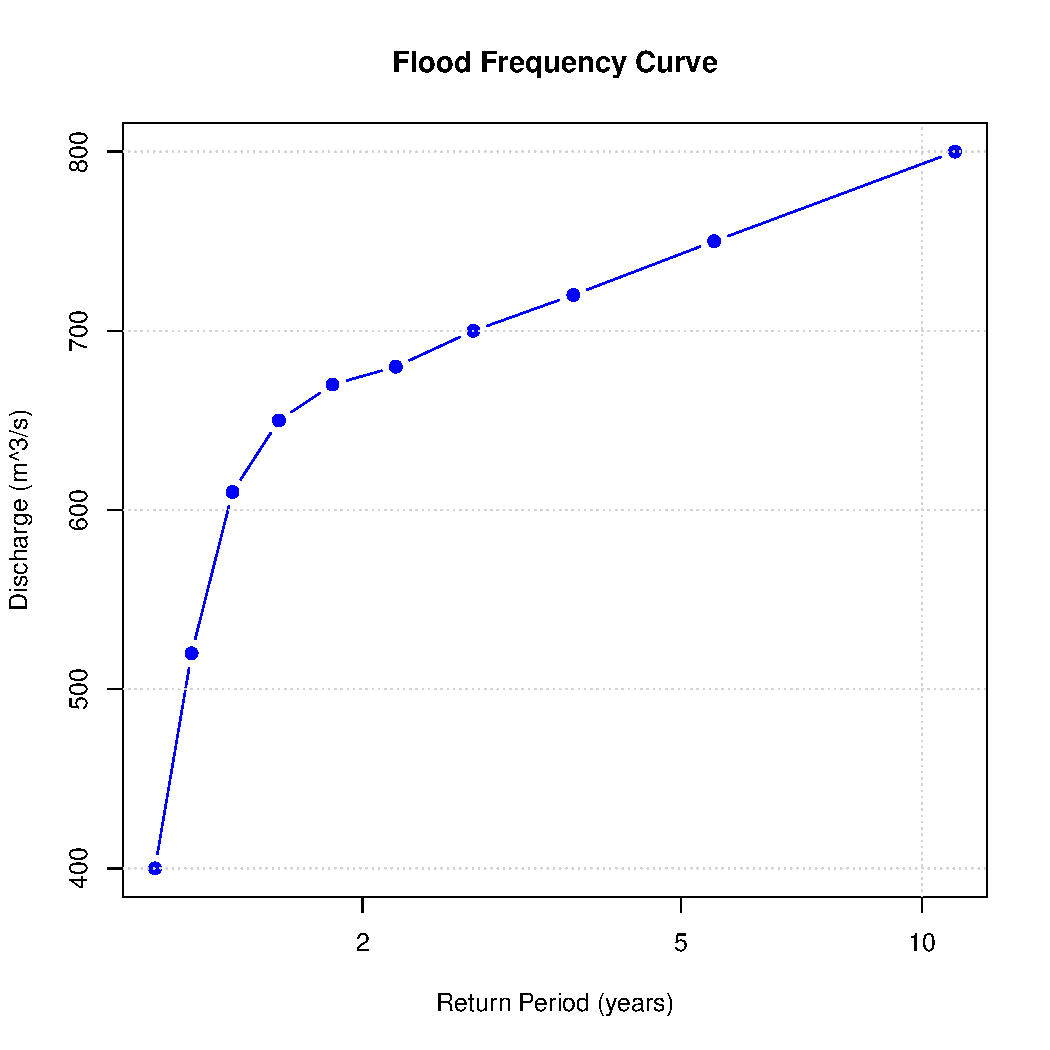
\includegraphics[width=\maxwidth]{figure/flood_plot-1} 
\end{knitrout}


\section{Using USGS Data}

\subsection{Load Required Packages}
\begin{knitrout}
\definecolor{shadecolor}{rgb}{0.969, 0.969, 0.969}\color{fgcolor}\begin{kframe}
\begin{alltt}
\hlcom{### STEP 1}


\hlcom{### STEP 2}
\hlcom{### Loading two specific packages into RWater}
\hlkwd{library}\hlstd{(dataRetrieval)}
\hlkwd{library}\hlstd{(xts)}
\end{alltt}


{\ttfamily\noindent\itshape\color{messagecolor}{\#\# Loading required package: zoo}}

{\ttfamily\noindent\itshape\color{messagecolor}{\#\# \\\#\# Attaching package: 'zoo'}}

{\ttfamily\noindent\itshape\color{messagecolor}{\#\# The following objects are masked from 'package:base':\\\#\# \\\#\# \ \ \ \ as.Date, as.Date.numeric}}\end{kframe}
\end{knitrout}

\subsection{Load Data}

\begin{knitrout}
\definecolor{shadecolor}{rgb}{0.969, 0.969, 0.969}\color{fgcolor}\begin{kframe}
\begin{alltt}
\hlcom{### STEP 3}
\hlcom{### Get the Peak Annual Discharge}
\hlstd{mysite} \hlkwb{<-} \hlstr{"07061000"}
\hlstd{startDate} \hlkwb{=} \hlstr{""}
\hlstd{endDate} \hlkwb{=} \hlstr{""}
\hlstd{annualpeak}\hlkwb{<-}\hlkwd{readNWISpeak}\hlstd{(mysite, startDate, endDate)}
\hlstd{Qmax_2025} \hlkwb{=} \hlnum{179000} \hlcom{#4/5/2025 11 CDT}

\hlkwd{names}\hlstd{(annualpeak)[}\hlnum{1}\hlopt{:}\hlnum{5}\hlstd{]}
\end{alltt}
\begin{verbatim}
## [1] "agency_cd" "site_no"   "peak_dt"   "peak_tm"  
## [5] "peak_va"
\end{verbatim}
\end{kframe}
\end{knitrout}


\subsection{Plot Data}

\begin{knitrout}
\definecolor{shadecolor}{rgb}{0.969, 0.969, 0.969}\color{fgcolor}\begin{kframe}
\begin{alltt}
\hlcom{### STEP 4}
\hlcom{### Plot the data}
\hlkwd{par}\hlstd{(}\hlkwc{mfrow}\hlstd{=}\hlkwd{c}\hlstd{(}\hlnum{1}\hlstd{,}\hlnum{1}\hlstd{))}
\hlkwd{plot}\hlstd{(annualpeak}\hlopt{$}\hlstd{peak_dt, annualpeak}\hlopt{$}\hlstd{peak_va,} \hlkwc{type}\hlstd{=}\hlstr{"p"}\hlstd{,} \hlkwc{pch}\hlstd{=}\hlnum{19}\hlstd{,} \hlkwc{cex}\hlstd{=}\hlnum{.7}\hlstd{,} \hlkwc{col}\hlstd{=}\hlstr{"blue"}\hlstd{,}
     \hlkwc{xlab}\hlstd{=}\hlstr{"Date"}\hlstd{,} \hlkwc{ylab}\hlstd{=}\hlstr{"Peak Discharge (cfs)"}\hlstd{,} \hlkwc{main}\hlstd{=}\hlstr{"Annual Peak Discharge"}\hlstd{)}
\hlkwd{abline}\hlstd{(}\hlkwc{h}\hlstd{=Qmax_2025,} \hlkwc{col}\hlstd{=}\hlstr{"red"}\hlstd{,} \hlkwc{lty}\hlstd{=}\hlnum{2}\hlstd{)}
\hlkwd{legend}\hlstd{(}\hlstr{"topright"}\hlstd{,} \hlkwc{legend}\hlstd{=}\hlkwd{c}\hlstd{(}\hlstr{"Annual Peak Discharge"}\hlstd{,} \hlstr{"2025 Qmax"}\hlstd{),}
       \hlkwc{col}\hlstd{=}\hlkwd{c}\hlstd{(}\hlstr{"blue"}\hlstd{,} \hlstr{"red"}\hlstd{),} \hlkwc{pch}\hlstd{=}\hlkwd{c}\hlstd{(}\hlnum{19}\hlstd{,} \hlnum{NA}\hlstd{),} \hlkwc{cex} \hlstd{=} \hlnum{.7}\hlstd{,} \hlkwc{lty}\hlstd{=}\hlkwd{c}\hlstd{(}\hlnum{NA}\hlstd{,} \hlnum{2}\hlstd{))}
\end{alltt}
\end{kframe}
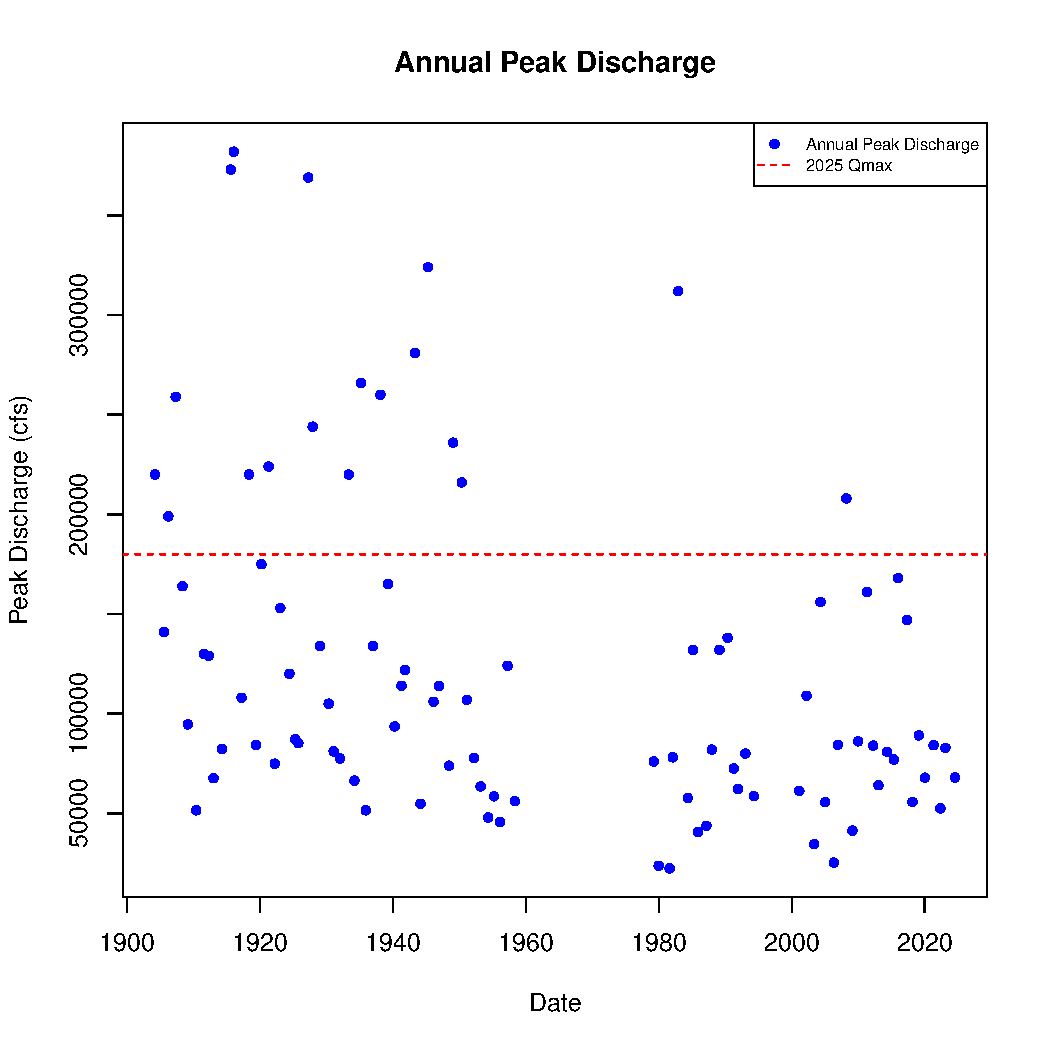
\includegraphics[width=\maxwidth]{figure/unnamed-chunk-7-1} 
\end{knitrout}



\subsection{Determine Station Records Ranges ()}


\begin{knitrout}
\definecolor{shadecolor}{rgb}{0.969, 0.969, 0.969}\color{fgcolor}\begin{kframe}
\begin{alltt}
\hlstd{annualpeak} \hlkwb{=} \hlstd{annualpeak[}\hlkwd{complete.cases}\hlstd{(annualpeak}\hlopt{$}\hlstd{peak_va),]}
\hlstd{annualpeak} \hlkwb{=} \hlstd{annualpeak[}\hlkwd{complete.cases}\hlstd{(annualpeak}\hlopt{$}\hlstd{peak_dt),]}
\hlstd{dt_range} \hlkwb{=} \hlkwd{range}\hlstd{(annualpeak}\hlopt{$}\hlstd{peak_dt);dt_range}
\end{alltt}
\begin{verbatim}
## [1] "1904-03-27" "2024-07-18"
\end{verbatim}
\begin{alltt}
\hlstd{va_range} \hlkwb{=} \hlkwd{range}\hlstd{(annualpeak}\hlopt{$}\hlstd{peak_va); va_range}
\end{alltt}
\begin{verbatim}
## [1]  22400 382000
\end{verbatim}
\end{kframe}
\end{knitrout}

\subsection{Split Data into Two Periods}

\begin{knitrout}
\definecolor{shadecolor}{rgb}{0.969, 0.969, 0.969}\color{fgcolor}\begin{kframe}
\begin{alltt}
\hlcom{### STEP 4}
\hlcom{### Split the downloaded data into two periods}
\hlstd{period1} \hlkwb{<-}\hlkwd{subset}\hlstd{(annualpeak, peak_dt}\hlopt{>=}\hlstd{dt_range[}\hlnum{1}\hlstd{]} \hlopt{&} \hlstd{peak_dt}\hlopt{<=}\hlstr{"2010-12-31"}\hlstd{)}
\hlstd{period2} \hlkwb{<-}\hlkwd{subset}\hlstd{(annualpeak, peak_dt}\hlopt{>=}\hlstr{"2010-12-31"} \hlopt{&} \hlstd{peak_dt}\hlopt{<=}\hlstd{dt_range[}\hlnum{2}\hlstd{])}
\end{alltt}
\end{kframe}
\end{knitrout}


\begin{knitrout}
\definecolor{shadecolor}{rgb}{0.969, 0.969, 0.969}\color{fgcolor}\begin{kframe}
\begin{alltt}
\hlcom{## NOT RUN -- just an example}
\hlcom{### STEP 5}
\hlcom{### Split the plot window in two columns}
\hlkwd{par}\hlstd{(}\hlkwc{mfrow}\hlstd{=}\hlkwd{c}\hlstd{(}\hlnum{1}\hlstd{,}\hlnum{2}\hlstd{))}

\hlkwd{plot}\hlstd{(period1}\hlopt{$}\hlstd{peak_dt, period1}\hlopt{$}\hlstd{peak_va,} \hlkwc{type}\hlstd{=}\hlstr{"p"}\hlstd{,} \hlkwc{pch}\hlstd{=}\hlnum{19}\hlstd{,}
     \hlkwc{col}\hlstd{=}\hlstr{"blue"}\hlstd{,} \hlkwc{xlab}\hlstd{=}\hlstr{"Date"}\hlstd{,} \hlkwc{ylab}\hlstd{=}\hlstr{"Peak Discharge (cfs)"}\hlstd{,} \hlkwc{main}\hlstd{=}\hlstr{"Period 1"}\hlstd{)}
\hlkwd{plot}\hlstd{(period2}\hlopt{$}\hlstd{peak_dt, period2}\hlopt{$}\hlstd{peak_va,} \hlkwc{type}\hlstd{=}\hlstr{"p"}\hlstd{,} \hlkwc{pch}\hlstd{=}\hlnum{19}\hlstd{,}
     \hlkwc{col}\hlstd{=}\hlstr{"red"}\hlstd{,} \hlkwc{xlab}\hlstd{=}\hlstr{"Date"}\hlstd{,} \hlkwc{ylab}\hlstd{=}\hlstr{"Peak Discharge (cfs)"}\hlstd{,} \hlkwc{main}\hlstd{=}\hlstr{"Period 2"}\hlstd{)}
\hlcom{### Add a legend}
\hlkwd{legend}\hlstd{(}\hlstr{"topright"}\hlstd{,} \hlkwc{legend}\hlstd{=}\hlkwd{c}\hlstd{(}\hlstr{"Period 1"}\hlstd{,} \hlstr{"Period 2"}\hlstd{),}
       \hlkwc{col}\hlstd{=}\hlkwd{c}\hlstd{(}\hlstr{"blue"}\hlstd{,} \hlstr{"red"}\hlstd{),} \hlkwc{pch}\hlstd{=}\hlnum{19}\hlstd{)}
\end{alltt}
\end{kframe}
\end{knitrout}


\begin{figure*}
\begin{knitrout}
\definecolor{shadecolor}{rgb}{0.969, 0.969, 0.969}\color{fgcolor}\begin{kframe}
\begin{alltt}
\hlcom{# Added ylim for the figures to match}
\hlkwd{par}\hlstd{(}\hlkwc{mfrow}\hlstd{=}\hlkwd{c}\hlstd{(}\hlnum{1}\hlstd{,}\hlnum{2}\hlstd{))}

\hlkwd{plot}\hlstd{(period1}\hlopt{$}\hlstd{peak_dt, period1}\hlopt{$}\hlstd{peak_va,} \hlkwc{type}\hlstd{=}\hlstr{"p"}\hlstd{,} \hlkwc{pch}\hlstd{=}\hlnum{19}\hlstd{,}
     \hlkwc{col}\hlstd{=}\hlstr{"blue"}\hlstd{,} \hlkwc{xlab}\hlstd{=}\hlstr{"Date"}\hlstd{,} \hlkwc{ylab}\hlstd{=}\hlstr{"Peak Discharge (cfs)"}\hlstd{,}
     \hlkwc{main}\hlstd{=}\hlstr{"Period 1"}\hlstd{,} \hlkwc{ylim}\hlstd{=}\hlkwd{c}\hlstd{(}\hlnum{0}\hlstd{, va_range[}\hlnum{2}\hlstd{]))}
\hlkwd{plot}\hlstd{(period2}\hlopt{$}\hlstd{peak_dt, period2}\hlopt{$}\hlstd{peak_va,} \hlkwc{type}\hlstd{=}\hlstr{"p"}\hlstd{,} \hlkwc{pch}\hlstd{=}\hlnum{19}\hlstd{,}
     \hlkwc{col}\hlstd{=}\hlstr{"red"}\hlstd{,} \hlkwc{xlab}\hlstd{=}\hlstr{"Date"}\hlstd{,} \hlkwc{ylab}\hlstd{=}\hlstr{"Peak Discharge (cfs)"}\hlstd{,}
     \hlkwc{main}\hlstd{=}\hlstr{"Period 2"}\hlstd{,} \hlkwc{ylim}\hlstd{=}\hlkwd{c}\hlstd{(}\hlnum{0}\hlstd{, va_range[}\hlnum{2}\hlstd{]))}
\hlcom{### Add a legend}
\hlkwd{legend}\hlstd{(}\hlstr{"topright"}\hlstd{,} \hlkwc{legend}\hlstd{=}\hlkwd{c}\hlstd{(}\hlstr{"Period 1"}\hlstd{,} \hlstr{"Period 2"}\hlstd{),}
       \hlkwc{col}\hlstd{=}\hlkwd{c}\hlstd{(}\hlstr{"blue"}\hlstd{,} \hlstr{"red"}\hlstd{),} \hlkwc{pch}\hlstd{=}\hlnum{19}\hlstd{)}
\end{alltt}
\end{kframe}
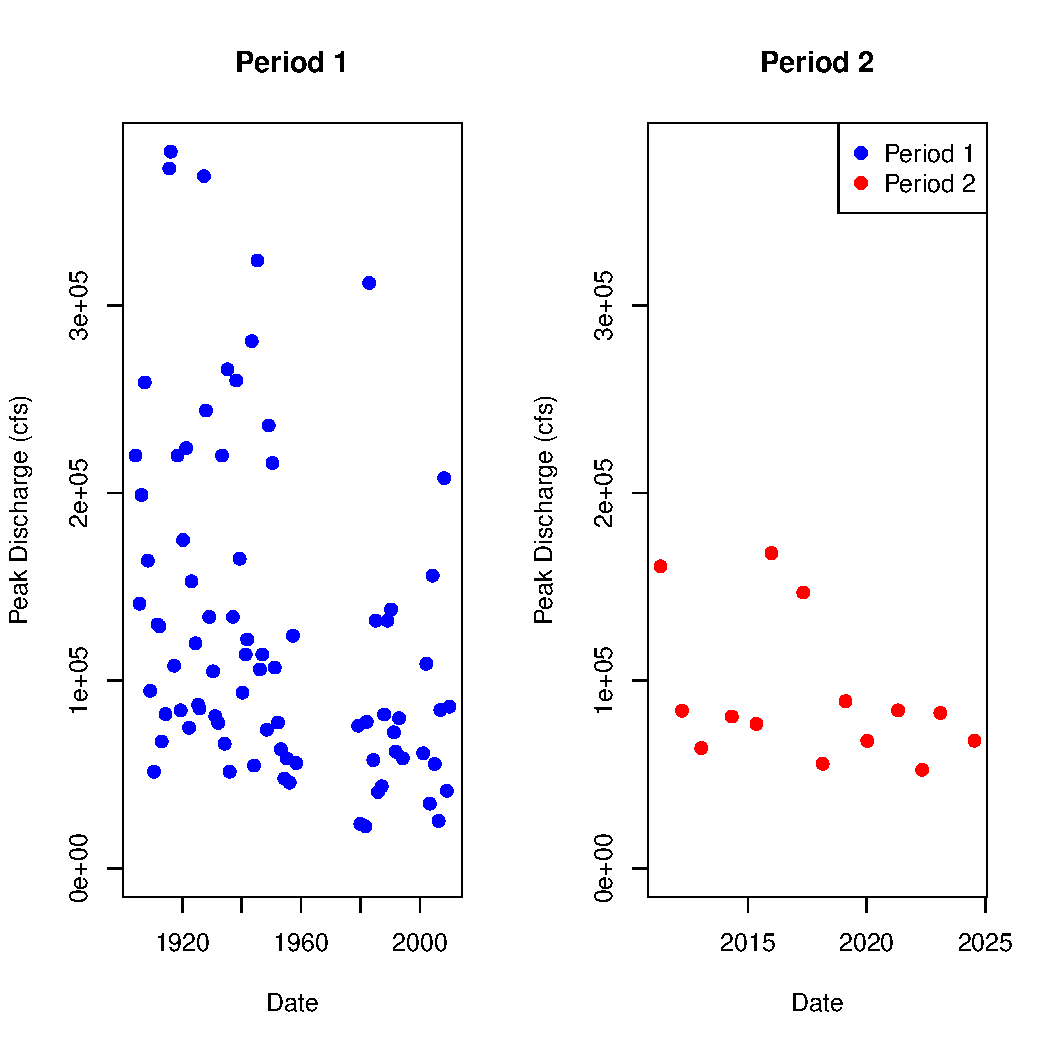
\includegraphics[width=\maxwidth]{figure/unnamed-chunk-11-1} 
\end{knitrout}
\end{figure*}

\subsection{Fit Peak Flow with `Method of Moments`}





\begin{knitrout}
\definecolor{shadecolor}{rgb}{0.969, 0.969, 0.969}\color{fgcolor}\begin{kframe}
\begin{alltt}
\hlcom{### STEP 6}
\hlcom{### Perform Flood Frequency Analysis }
\hlcom{### Locate the column of your data set that has the peak discharges}
\hlcom{### You can see that peak discharges are stored in the 6th column (peak_va)}

\hlstd{Q} \hlkwb{=} \hlstd{period1}\hlopt{$}\hlstd{peak_va}
\hlcom{# extract year from date range??}
\hlcom{# Q$peak_dt = as.Date(period1$peak_dt, format="%Y")}

\hlcom{# format(as.Date(period1$peak_dt, format="%d/%m/%Y"),"%Y")}
\hlstd{graphlab} \hlkwb{=} \hlkwd{paste}\hlstd{(}\hlkwd{range}\hlstd{(}\hlkwd{format}\hlstd{(}\hlkwd{as.Date}\hlstd{(period1}\hlopt{$}\hlstd{peak_dt,} \hlkwc{format}\hlstd{=}\hlstr{"%d/%m/%Y"}\hlstd{),}\hlstr{"%Y"}\hlstd{)),} \hlkwc{collapse} \hlstd{=} \hlstr{"-"}\hlstd{)}

\hlcom{# Generate plotting positions}
\hlstd{n} \hlkwb{=} \hlkwd{length}\hlstd{(Q); n}
\end{alltt}
\begin{verbatim}
## [1] 81
\end{verbatim}
\begin{alltt}
\hlstd{r} \hlkwb{=} \hlstd{n} \hlopt{+} \hlnum{1} \hlopt{-} \hlkwd{rank}\hlstd{(Q);} \hlkwd{head}\hlstd{(r)}  \hlcom{# highest Q has rank r = 1}
\end{alltt}
\begin{verbatim}
## [1] 14 24 18  9 21 42
\end{verbatim}
\begin{alltt}
\hlstd{T} \hlkwb{=} \hlstd{(n} \hlopt{+} \hlnum{1}\hlstd{)}\hlopt{/}\hlstd{r;} \hlkwd{head}\hlstd{(T)}
\end{alltt}
\begin{verbatim}
## [1] 5.857143 3.416667 4.555556 9.111111 3.904762 1.952381
\end{verbatim}
\begin{alltt}
\hlcom{# Set up x axis tick positions and labels}
\hlstd{Ttick} \hlkwb{=} \hlkwd{c}\hlstd{(}\hlnum{1.001}\hlstd{,}\hlnum{1.01}\hlstd{,}\hlnum{1.1}\hlstd{,}\hlnum{1.5}\hlstd{,}\hlnum{2}\hlstd{,}\hlnum{3}\hlstd{,}\hlnum{4}\hlstd{,}\hlnum{5}\hlstd{,}\hlnum{6}\hlstd{,}\hlnum{7}\hlstd{,}\hlnum{8}\hlstd{,}\hlnum{9}\hlstd{,}\hlnum{10}\hlstd{,}\hlnum{11}\hlstd{,}\hlnum{12}\hlstd{,}\hlnum{13}\hlstd{,}
          \hlnum{14}\hlstd{,}\hlnum{15}\hlstd{,}\hlnum{16}\hlstd{,}\hlnum{17}\hlstd{,}\hlnum{18}\hlstd{,}\hlnum{19}\hlstd{,}\hlnum{20}\hlstd{,}\hlnum{25}\hlstd{,}\hlnum{30}\hlstd{,}\hlnum{35}\hlstd{,}\hlnum{40}\hlstd{,}\hlnum{45}\hlstd{,}\hlnum{50}\hlstd{,}\hlnum{60}\hlstd{,}\hlnum{70}\hlstd{,}\hlnum{80}\hlstd{,}\hlnum{90}\hlstd{,}\hlnum{100}\hlstd{)}
\hlstd{xtlab} \hlkwb{=} \hlkwd{c}\hlstd{(}\hlnum{1.001}\hlstd{,}\hlnum{1.01}\hlstd{,}\hlnum{1.1}\hlstd{,}\hlnum{1.5}\hlstd{,}\hlnum{2}\hlstd{,}\hlnum{NA}\hlstd{,}\hlnum{NA}\hlstd{,}\hlnum{5}\hlstd{,}\hlnum{NA}\hlstd{,}\hlnum{NA}\hlstd{,}\hlnum{NA}\hlstd{,}\hlnum{NA}\hlstd{,}\hlnum{10}\hlstd{,}\hlnum{NA}\hlstd{,}
          \hlnum{NA}\hlstd{,}\hlnum{NA}\hlstd{,}\hlnum{NA}\hlstd{,}\hlnum{15}\hlstd{,}\hlnum{NA}\hlstd{,}\hlnum{NA}\hlstd{,}\hlnum{NA}\hlstd{,}\hlnum{NA}\hlstd{,}\hlnum{20}\hlstd{,}\hlnum{NA}\hlstd{,}\hlnum{30}\hlstd{,}\hlnum{NA}\hlstd{,}\hlnum{NA}\hlstd{,}\hlnum{NA}\hlstd{,}\hlnum{50}\hlstd{,}\hlnum{NA}\hlstd{,}\hlnum{NA}\hlstd{,}\hlnum{NA}\hlstd{,}\hlnum{NA}\hlstd{,}\hlnum{100}\hlstd{)}
\hlstd{y} \hlkwb{=} \hlopt{-}\hlkwd{log}\hlstd{(}\hlopt{-}\hlkwd{log}\hlstd{(}\hlnum{1} \hlopt{-} \hlnum{1}\hlopt{/}\hlstd{T))}
\hlstd{ytick} \hlkwb{=} \hlopt{-}\hlkwd{log}\hlstd{(}\hlopt{-}\hlkwd{log}\hlstd{(}\hlnum{1} \hlopt{-} \hlnum{1}\hlopt{/}\hlstd{Ttick))}
\hlstd{xmin} \hlkwb{=} \hlkwd{min}\hlstd{(}\hlkwd{min}\hlstd{(y),}\hlkwd{min}\hlstd{(ytick))}
\hlstd{xmax} \hlkwb{=} \hlkwd{max}\hlstd{(ytick)}

\hlcom{# Fit a line by method of moments, along with 95% confidence intervals}
\hlstd{KTtick} \hlkwb{=} \hlopt{-}\hlstd{(}\hlkwd{sqrt}\hlstd{(}\hlnum{6}\hlstd{)}\hlopt{/}\hlstd{pi)}\hlopt{*}\hlstd{(}\hlnum{0.5772} \hlopt{+} \hlkwd{log}\hlstd{(}\hlkwd{log}\hlstd{(Ttick}\hlopt{/}\hlstd{(Ttick}\hlopt{-}\hlnum{1}\hlstd{))))}
\hlstd{QTtick} \hlkwb{=} \hlkwd{mean}\hlstd{(Q)} \hlopt{+} \hlstd{KTtick}\hlopt{*}\hlkwd{sd}\hlstd{(Q)}
\hlstd{nQ} \hlkwb{=} \hlkwd{length}\hlstd{(Q)}
\hlstd{se} \hlkwb{=} \hlstd{(}\hlkwd{sd}\hlstd{(Q)}\hlopt{*}\hlkwd{sqrt}\hlstd{((}\hlnum{1}\hlopt{+}\hlnum{1.14}\hlopt{*}\hlstd{KTtick} \hlopt{+} \hlnum{1.1}\hlopt{*}\hlstd{KTtick}\hlopt{^}\hlnum{2}\hlstd{)))}\hlopt{/}\hlkwd{sqrt}\hlstd{(nQ)}
\hlstd{LB} \hlkwb{=} \hlstd{QTtick} \hlopt{-} \hlkwd{qt}\hlstd{(}\hlnum{0.975}\hlstd{, nQ} \hlopt{-} \hlnum{1}\hlstd{)}\hlopt{*}\hlstd{se}
\hlstd{UB} \hlkwb{=} \hlstd{QTtick} \hlopt{+} \hlkwd{qt}\hlstd{(}\hlnum{0.975}\hlstd{, nQ} \hlopt{-} \hlnum{1}\hlstd{)}\hlopt{*}\hlstd{se}
\hlstd{max} \hlkwb{=} \hlkwd{max}\hlstd{(UB)}
\hlstd{Qmax} \hlkwb{=} \hlkwd{max}\hlstd{(QTtick)}
\end{alltt}
\end{kframe}
\end{knitrout}

\begin{figure*}
\begin{knitrout}
\definecolor{shadecolor}{rgb}{0.969, 0.969, 0.969}\color{fgcolor}
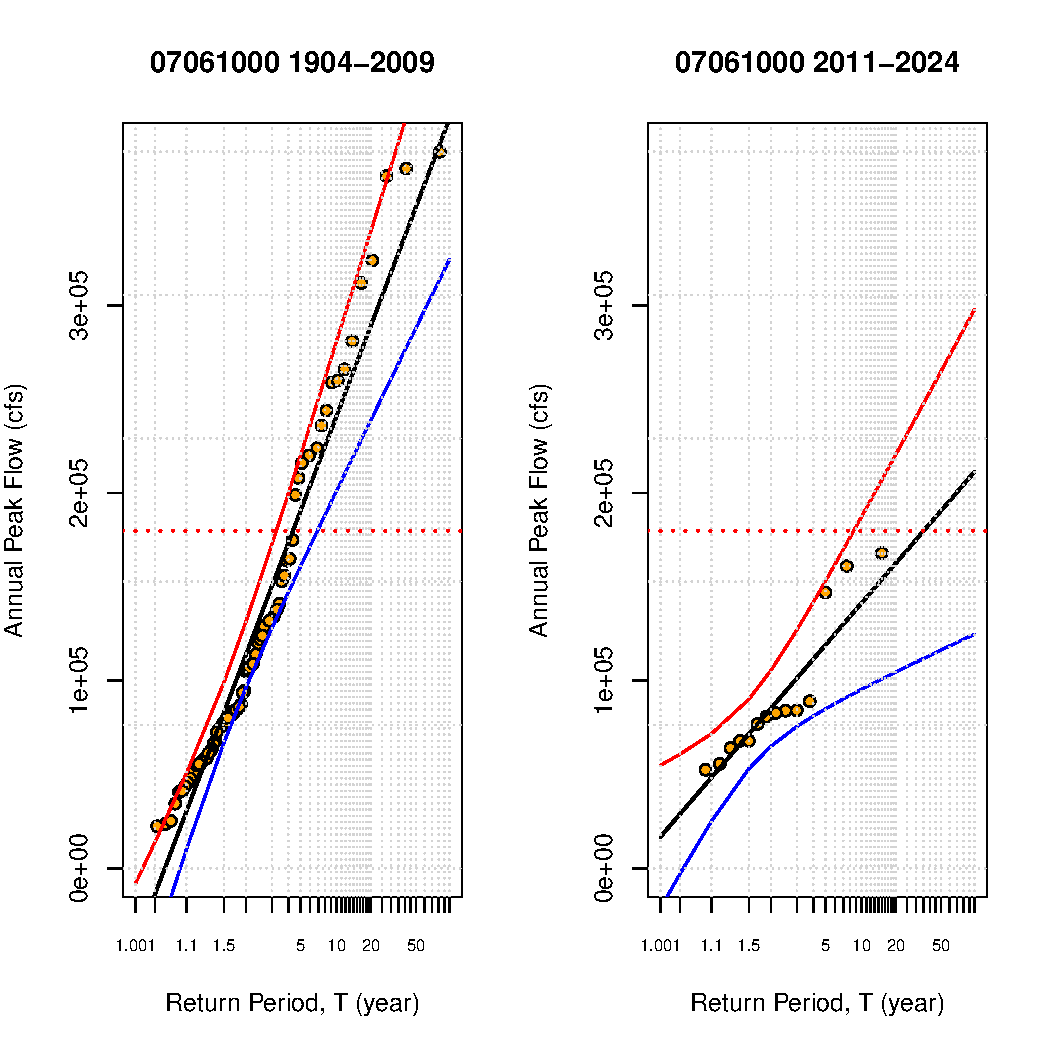
\includegraphics[width=\maxwidth]{figure/unnamed-chunk-13-1} 
\end{knitrout}
\end{figure*}


\begin{figure}
	\centering
		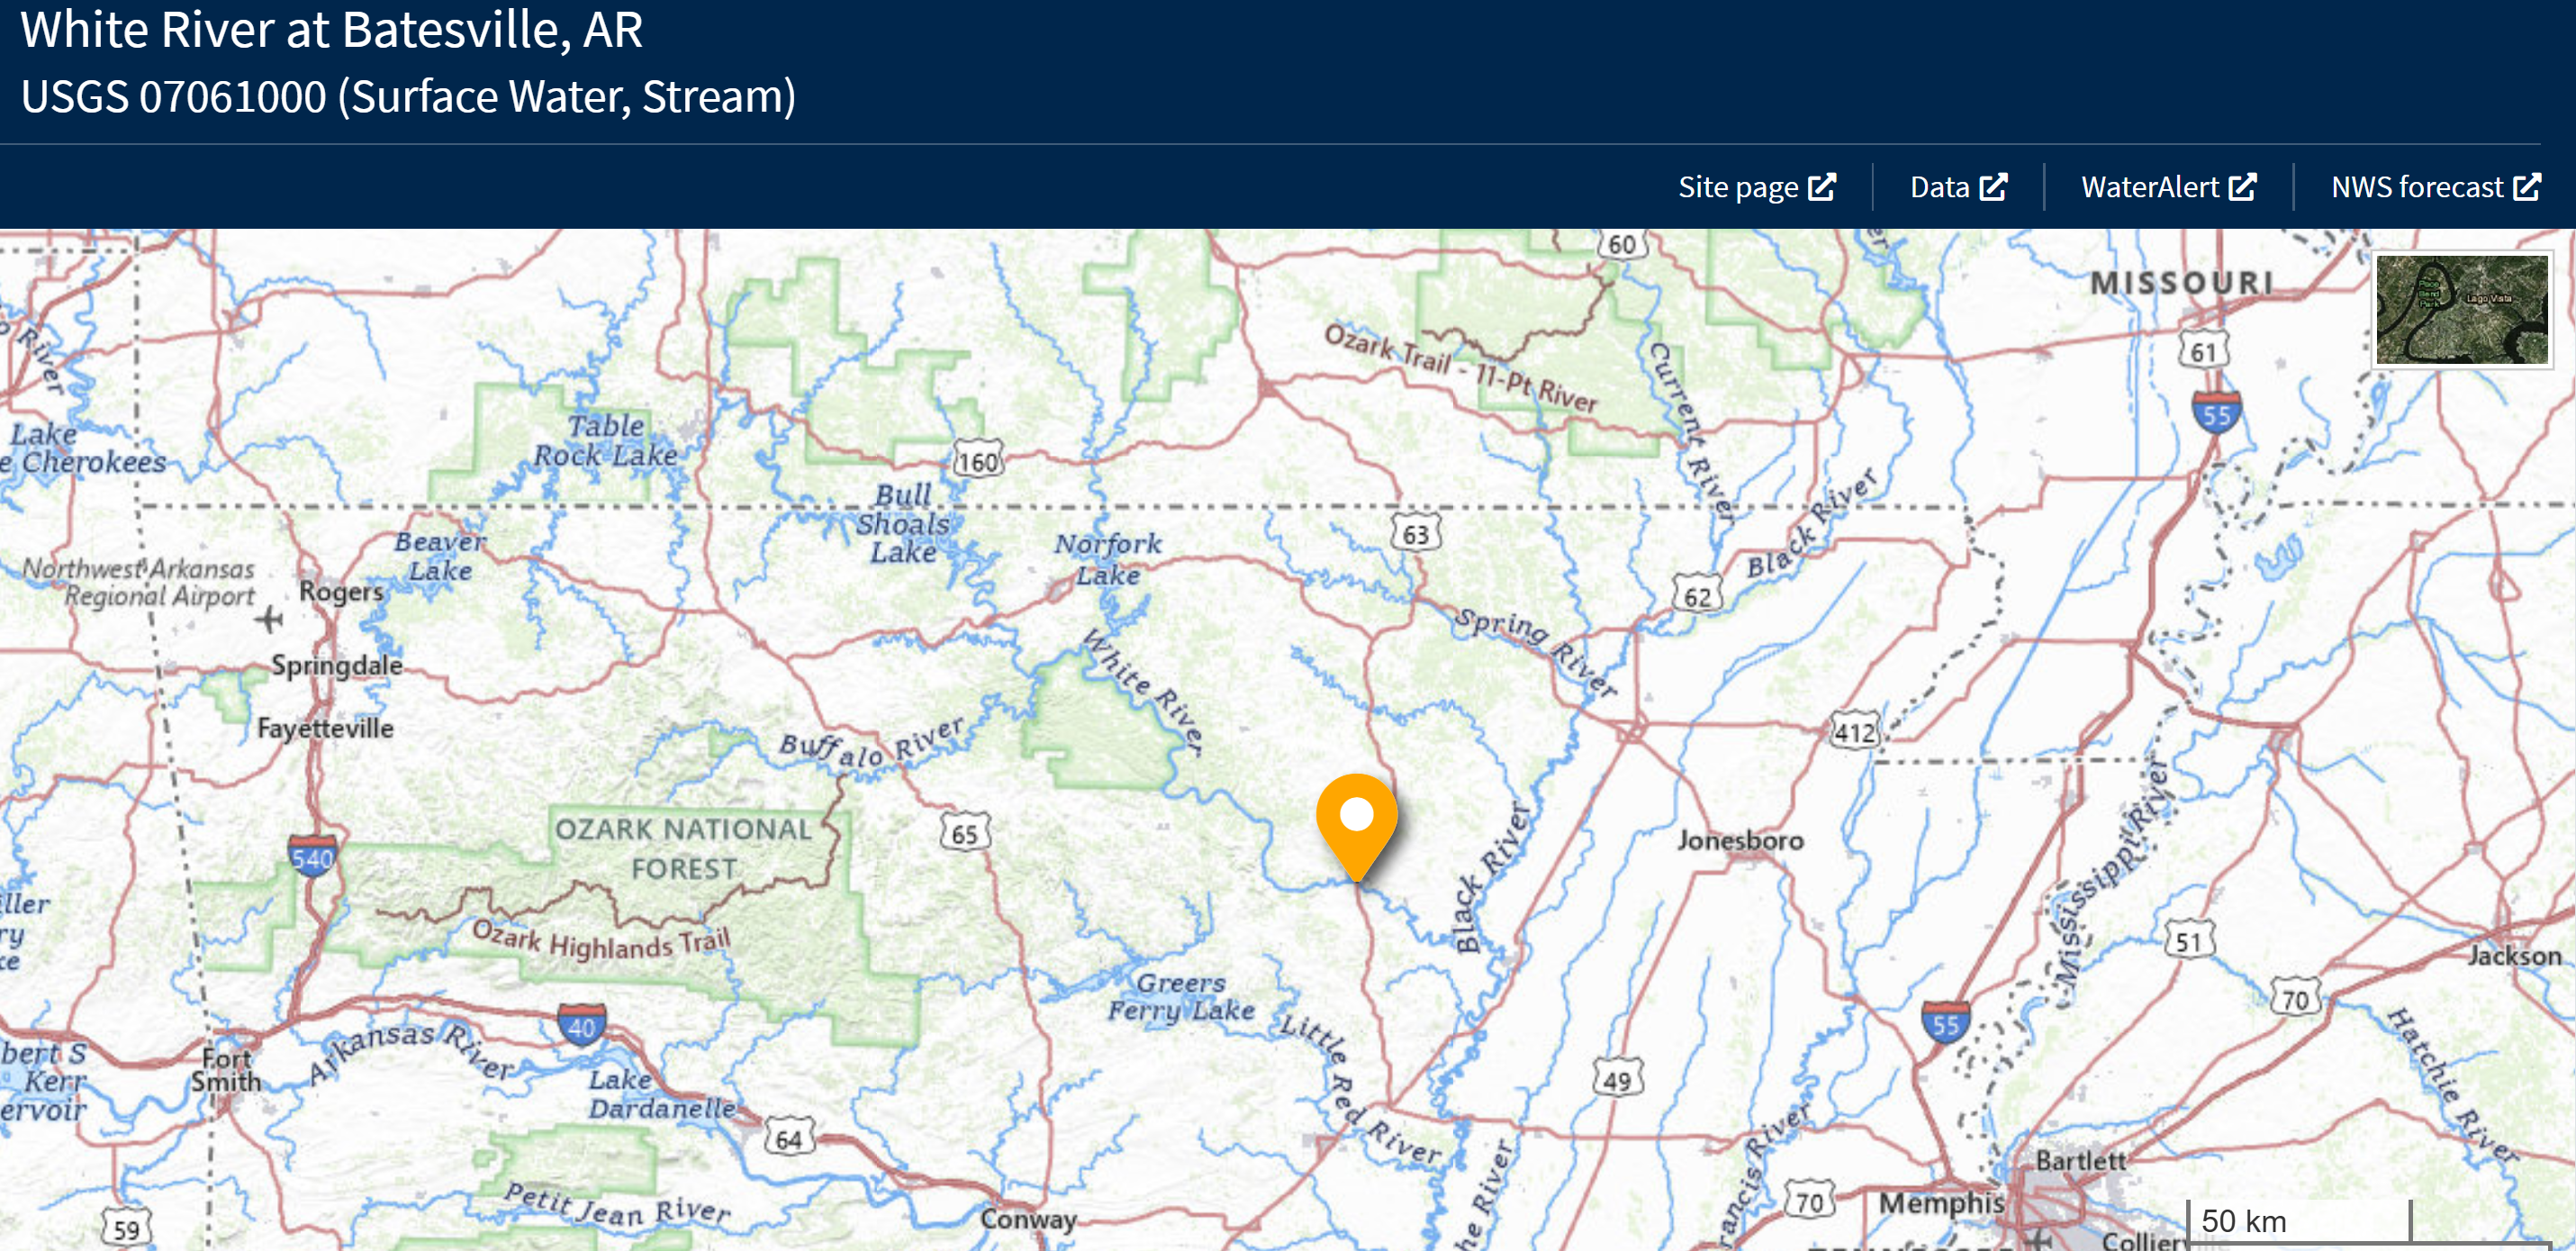
\includegraphics[width=1.00\textwidth]{figure/WhiteRiver.png}
		\caption{White River, Arkansas, USGS gage 07052500. Annual peak flow frequency analysis for the period 2000-2025 (left) and 1980-2000 (right). The red dashed line indicates the 2025 projected peak flow.}
	\label{fig:White River}
\end{figure}


\newpage
\addcontentsline{toc}{section}{References}
%\printbibliography
\bibliographystyle{apalike} 
%\renewcommand\bibname{References}{}
\bibliography{../references} % Use the references.bib file to create the bibliography	


\end{document}



